\section{Statistics}

\subsection{Causal Inference}

La inferencia causal es el proceso de determinar el \textbf{efecto independiente de una variable} en un sistema más complejo. En general, este proceso es necesario cuando buscamos obtener conclusiones de datos pasados y en los que no es posible realizar un \textit{A/B testing}.

Existen 3 desafíos al realizar este proceso: 
\begin{itemize}
    \item \textbf{Cofounders}: Son aquellas variables que tienen un impacto en el outcome y que incluso podrían tener un impacto en otras variables. 
    \item \textbf{Selection Bias}: Selección no representativa del grupo de control y tratamiento.
    \item \textbf{Counterfactuals}: Imputar valores en el grupo de control y tratamiento en base a \textit{Machine Learning} o algoritmos de \textit{Matching}. 
\end{itemize}

\begin{figure}[H]
    \center
    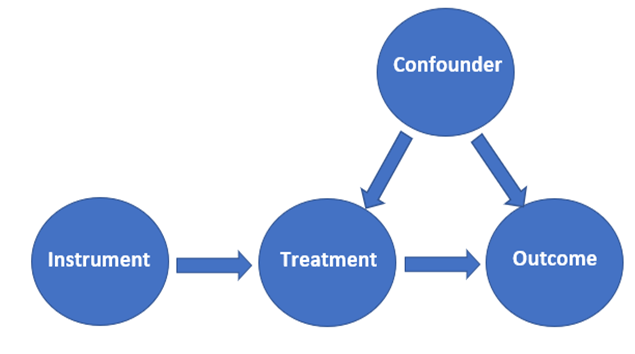
\includegraphics[scale=0.3]{notebooks/STATS/img/causal_inference_diagram.png}
    \caption{Casual Inference - DAG Diagram}
\end{figure}

Para resolver este problema, es necesario tomar algunos supuestos: 
\begin{enumerate}
    \item \textbf{Causal Markov Condition}: La influencia de las variables y el outcome puede ser representado a través de un \textbf{Grafo Acíclico Dirigido (DAG)} en el que se asume la \textbf{condición de Markov}, es decir si $Y \rightarrow S \rightarrow C$, podemos asumir que $C \indep Y | S$
    \item \textbf{SUTVA}: (Stable Unit Treatment Value Assumption) El grupo de control y tratamiento \textbf{no tiene influencia el uno con el otro}. 
    \item \textbf{Ignorability}: Se excluye el ruido proveniente de cualquier otra fuente. 
\end{enumerate}

Consideremos el siguiente ejemplo en el que buscamos determinar si el efecto de un tratamiento tiene un impacto en una variable target. 

\begin{figure}[H]
    \center
    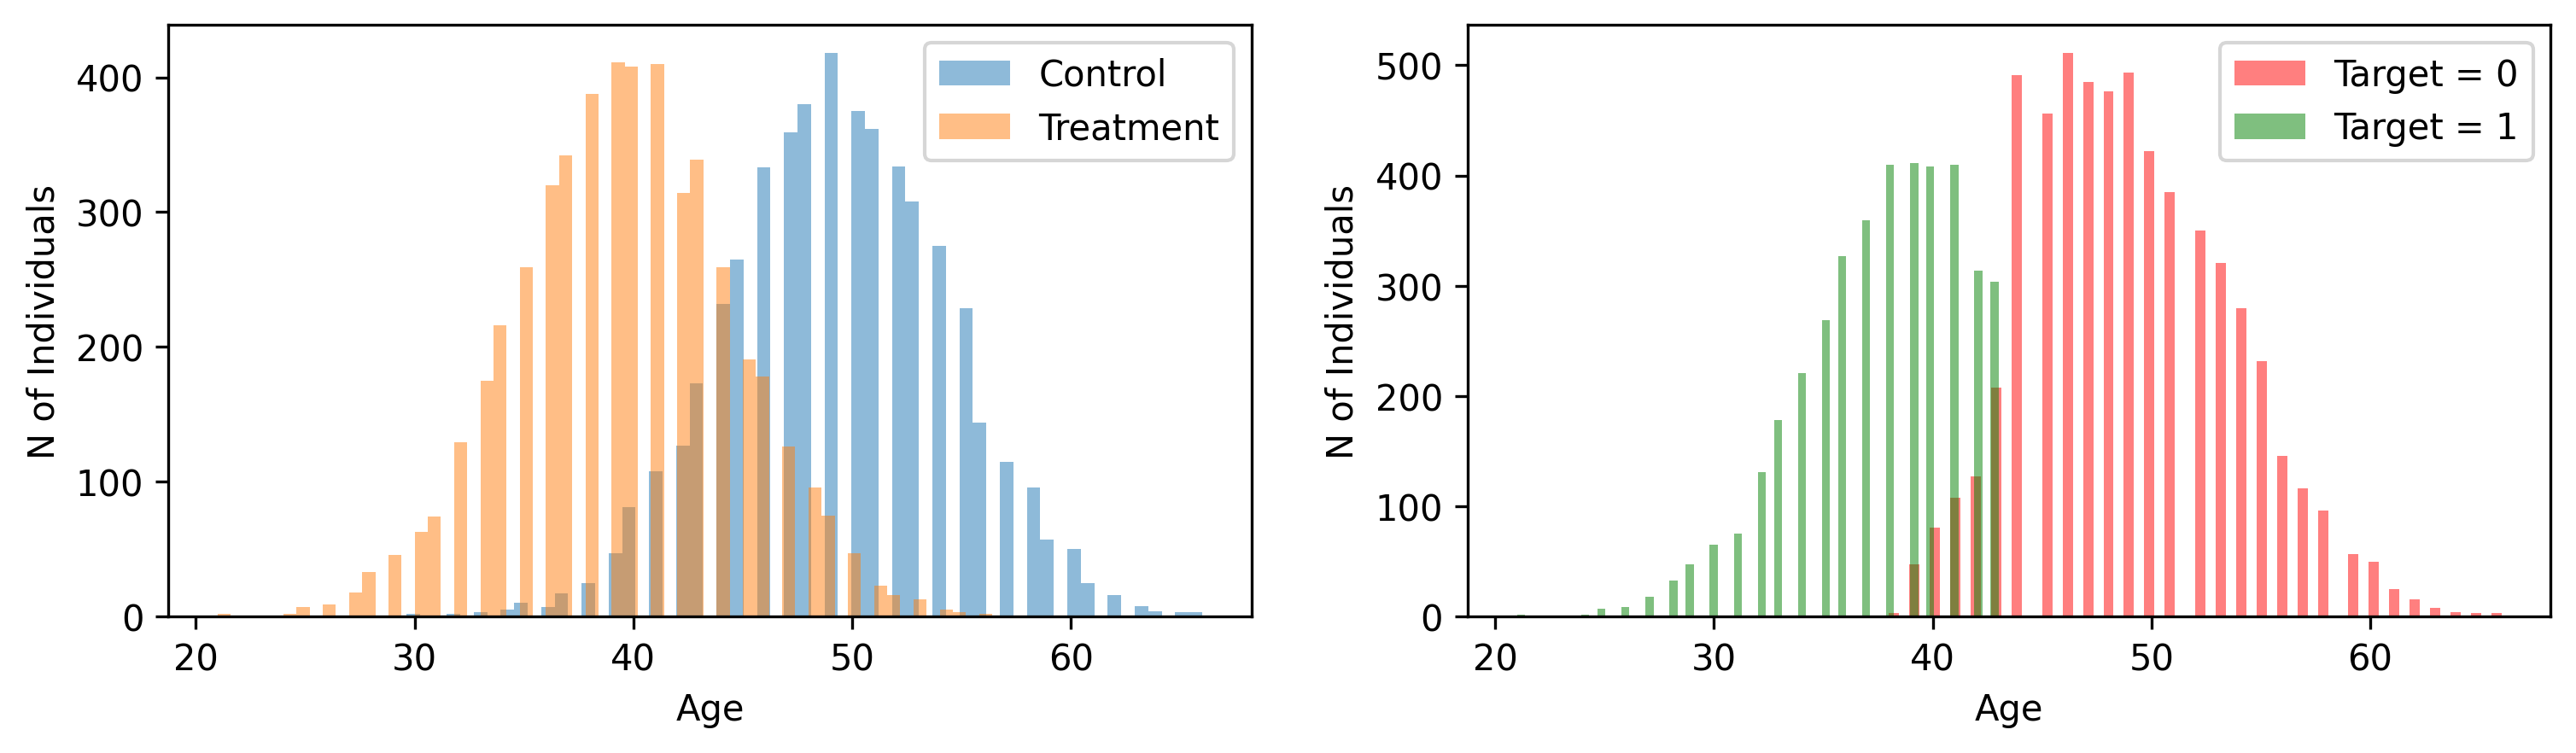
\includegraphics[scale=0.5]{notebooks/STATS/img/causal_inference_age_distribution.png}
    \caption{Casual Inference - Distribution Example}
\end{figure}

Vemos que existe un \textit{selection bias} pues el grupo de tratamiento y control tienen distribuciones de edad distintas. Existen múltiples enfoques para resolver este problema. 

\subsubsection{Matching Imputation}

Es posible utilizar un algoritmo de \textit{Matching} como \textit{NearestNeighbors} para imputar el posible outcome que hubiese tenido un individuo al recibir o no el tratamiento. En nuestro ejemplo, para cada edad de los individuos del grupo de control, buscaríamos al sujeto con la edad más cercana en el grupo de tratamiento e imputaríamos su respuesta al tratamiento y viceversa. 

La efectividad del tratamiento se puede medir a través del promedio de los outcome cuando reciben y cuando no reciben el tratamiento. 

\subsubsection{Meta Learners}

Este enfoque plantea utilizar algoritmos de \textit{Machine Learning} para determinar el efecto del tratamiento en el outcome del experimento. Sea $y_i$ el target, $w$ si recibió el tratamiento y $X_i$ el conjunto de variables del modelo, definimos ITE (\textit{Individual Treatment Effect}) según 
$$
\text{ITE} = \left [ p(y_i = 1 | w_i = 1, X_i) - p(y_i = 1 | w_i = 0, X_i) \right ]
$$

\begin{itemize}
    \item \textbf{S - Model} Este algoritmo es el más simple de todos pues agrega la variable \textit{treatment} como input de un único modelo. El valor de ITE es calculado para cada individuo variando el valor del tratamiento. 
    \item \textbf{T - Model} Este algoritmo entrena 2 clasificadores, uno encargado del grupo de control y otro para el grupo de tratamiento. El valor de ITE es calculado como la resta del output de ambos modelos. 

    Hay que tener en consideración que este modelo requiere una \textbf{calibración} para asegurar que el output de los modelos sean probabilidades.
    \item \textbf{X - Model}: SOON 
\end{itemize}


\begin{figure}[H]
    \center
    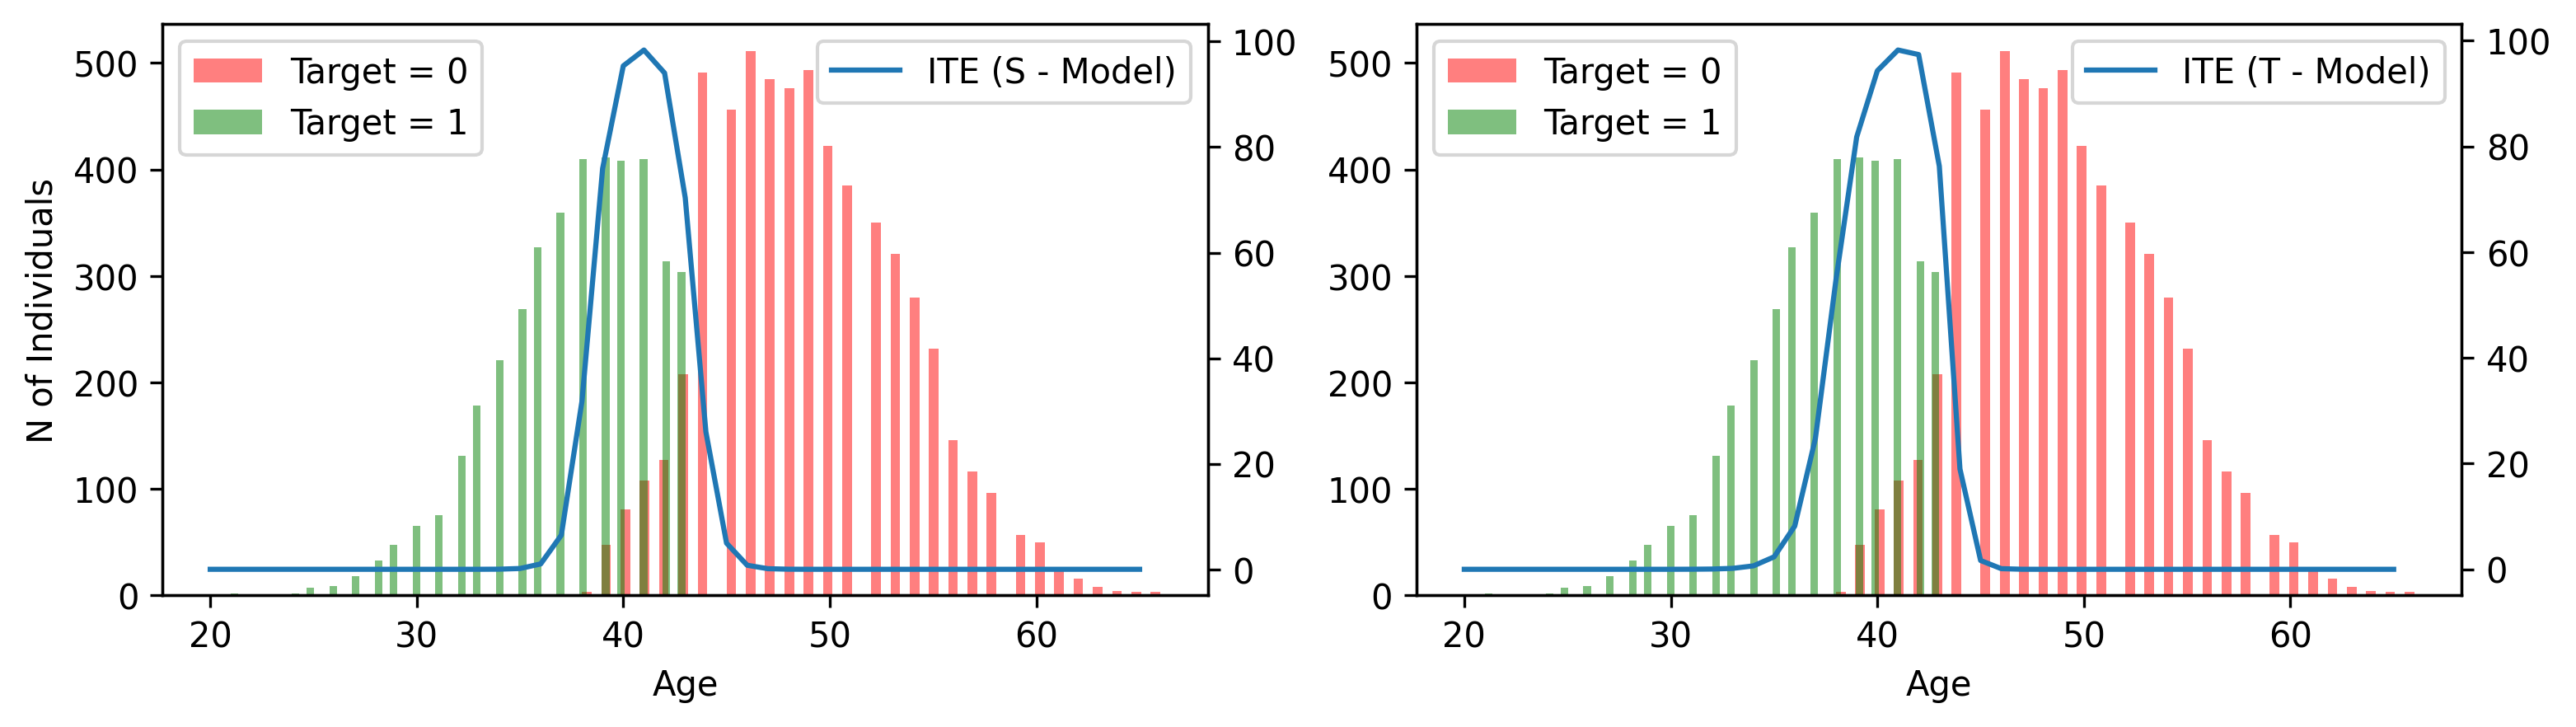
\includegraphics[scale=0.5]{notebooks/STATS/img/causal_inference_meta_learners.png}
    \caption{Meta Learners}
\end{figure}

Vemos así que el impacto del tratamiento aislando el efecto de la edad, ocurre según ITE entre los 35 y 45 años. 





